% Gemini theme
% https://github.com/anishathalye/gemini

\documentclass[final]{beamer}

% ====================
% Packages
% ====================

\usepackage[T1]{fontenc}
\usepackage{lmodern}
\usepackage[size=custom,width=121.92,height=91.44,scale=1.2]{beamerposter}
\usetheme{gemini}
\usecolortheme{gemini}
\usepackage{graphicx}
\graphicspath{{images/}}
\usepackage{booktabs}
\usepackage{tikz}
\usepackage{pgfplots}
\pgfplotsset{compat=1.14}
\def\code#1{\texttt{#1}}

% ====================
% Lengths
% ====================

% If you have N columns, choose \sepwidth and \colwidth such that
% (N+1)*\sepwidth + N*\colwidth = \paperwidth
\newlength{\sepwidth}
\newlength{\colwidth}
\setlength{\sepwidth}{0.025\paperwidth}
\setlength{\colwidth}{0.3\paperwidth}

\newcommand{\separatorcolumn}{\begin{column}{\sepwidth}\end{column}}

% ====================
% Title
% ====================

\title{Twitter: A Commentary}

\author{Ishan Shah \and Michael Chen \and Rishi Ponnekanti \and Udai Jain}

\institute[shortinst]{The University of Texas at Austin}

% ====================
% Footer (optional)
% ====================

\footercontent{
  \href{https://twittercommentary.netlify.app/}{https://twittercommentary.netlify.app/} \hfill
  EE 461P – Data Science Principles \hfill
  \href{mailto:ishan0102@utexas.edu}{ishan0102@utexas.edu}}
% (can be left out to remove footer)

% ====================
% Logo (optional)
% ====================

% use this to include logos on the left and/or right side of the header:
% \logoright{\includegraphics[height=7cm]{logo1.pdf}}
% \logoleft{\includegraphics[height=7cm]{logo2.pdf}}

% ====================
% Body
% ====================

\begin{document}

\begin{frame}[t]
\begin{columns}[t]
\separatorcolumn

\begin{column}{\colwidth}

  \begin{block}{Problem}

    Twitter has grown rapidly in the last decade as a platform for sharing short-form written content. It’s used by individuals to share thoughts and jokes, academics to discuss research, and even governments as a primary form of communication. This project seeks to predict response sentiment on a tweet’s replies using the tweet’s content.

    This problem is relevant today since many creators want to gauge how their audience will respond to their content before publishing it. This can also be beneficial to organizations to help rephrase tweets that may be interpreted negatively to protect reputation. Finally, while this project will be focused on Twitter, the techniques can easily be applied to other major platforms like YouTube and Facebook, to help content creators gather insights.

  \end{block}

  \begin{block}{Data Source}

    Building a model to accurately predict reponse sentiment requires a large amount of data. Manually collecting enough tweets and replies with the Twitter API is not feasible due to the rate limit, so we used an existing dataset \cite{RETWEET} to train our model. The data was provided as a CSV file of 34,521 tweet IDs, each of which had a list of reply sentiments (positive, neutral, negative) totalling in 1,519,504 unique replies.
    
    Using this, we collected the tweet text for each tweet using the \code{GET statuses/show/:id} route of the Twitter API. This took around 11 hours since we had to comply with the rate limit of 900 requests / 15 minutes. We also computed sentiment scores by converting the reply sentiments to numerical values (positive=1, neutral=0, negative=-1) and taking the average. Lastly, we added a column with the number of replies to each tweet.

  \end{block}

  \begin{block}{Pre-Processing}

    Once we had each tweet's text, we performed the following pre-processing steps:

    \begin{itemize}
      \item \textbf{Remove whitespace:} Remove any excess whitespace using regular expressions.
      \item \textbf{Normalize case:} Convert all letters to lowercase.
      \item \textbf{Tokenize string:} Split the text into tokens by whitespace.
      \item \textbf{Remove stopwords}: Use NLTK's stopwords dataset \cite{NLTK} to remove common words like \code{the}, \code{and}, \code{to}, etc.
      \item \textbf{Lemmatize words}: Use NLTK's lemmatizer to convert words to their base form.
      \item \textbf{Remove punctuation:} Remove any words containing punctuation like \code{@} or \code{\#}, which show up frequently in tweets.
    \end{itemize}

    Finally, we're left with the following features:

    \begin{table}
      \centering
      \begin{tabular}{l r r}
        \toprule
        \textbf{Cleaned Tweet} & \textbf{Reply Sentiment} & \textbf{Reply Count}\\
        \midrule
        fox corporation owner fox news trying bully ro...	& -0.520000	& 150 \\
        folk hear cornovirus deal news heck doctor rec...	& -0.200000	& 45 \\
        news finally excited journey potential finding...	& 0.500000	& 6 \\
        good news person investigation novel coronavir...	& -0.250000	& 12 \\
        two avid golfer promised whoever died first wo...	& 0.166667	& 36 \\
        \bottomrule
      \end{tabular}
      \caption{Dataset containing the cleaned words in each tweet, the sentiment of the tweet's replies, and the number of replies.}
    \end{table}

  \end{block}

\end{column}

\separatorcolumn

\begin{column}{\colwidth}

  \begin{block}{Vectorization}

    Performing text vectorization is common in natural language processing as it allows for text to be represented as vectors of numbers, letting us perform linear algebra operations on them. We used Scikit-learn's \code{TfidfVectorizer}, which uses the term frequency–inverse document frequency (TF-IDF) model to determine which words are most relevant to each document.
    
    Let $t$ be some term in a document $d$. The TF-IDF score is computed with:

    \begin{align*}
      \textbf{TFIDF(t, d)} = \frac{\text{Frequency of } t \text{ in } d}{\text{Total words in } d}
                       \cdot \text{log}\left(\frac{\text{Total documents}}{\text{Documents containing } t}\right)
    \end{align*}

    This captures the importance of each term in a document (TF) relative to how frequently it occurs in other documents (IDF). This is critical because it helps us find words that are unique to documents, rather than words that are common to all documents like \code{the}, \code{and}, etc. We can now train machine learning models on the vector representations of these tweets.

  \end{block}

  \begin{block}{Machine Learning}

    We use XGBoost to train our model. Specifically, we used the \code{XGBRegressor} as we were trying to predict the sentiment score of a tweet's replies which can have a continuous value. This sentiment value was computed by taking the sum of the numeric score using the mapping previously define (positive=1, neutral=0, negative=-1), then normalizing by dividing by the total number of replies for that tweet. Additionally, we used \code{RandomizedSearchCV} to search for the best hyperparameters to achieve the best results with the dataset.

    We can visualize the model's performance treating the results of the model as a classification problem. If we take the sign of the average of the sentiment scores, we can treat the model as a binary classification problem. We can then plot the ROC curve to see how the model's performs in terms of getting the overall sentiment for a tweet. 

    \begin{figure}[h]
      \centering
      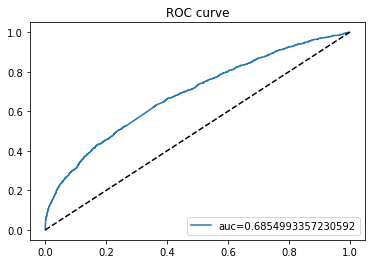
\includegraphics[width=0.6\textwidth]{auroc.png}
      \caption{ROC curve for the model on the training set.}
    \end{figure}

    This, however, is not a perfect metric since many tweets have a neutral sentiment that hovers relatively near 0; where taking the sign of such a tweet would not be a good indicator of the sentiment. The following plot shows the ROC curve for the model on the training set.

  \end{block}

\end{column}

\separatorcolumn

\begin{column}{\colwidth}

  \begin{alertblock}{Results}

    We tested our model on a subset of the data and found that the mean squared error on the best model was \textbf{0.1971}. Here are some takeaways this led us to:

    \begin{itemize}
      \item It is hard to judge the model's quality due to the nature of the data.
      \item While the model generally predicts the sentiment of the replies correctly, it was often swayed by certain words in the input with abnormally high prior probabilities.
      \item Sarcasm and humor are interpreted subjectively but machine learning models make objective predictions.
    \end{itemize}

    


  \end{alertblock}

  \begin{block}{Product Development}

    After training the model, we decided to build a simple webapp that would let users predict response sentiment on tweets of their own. We created a simple backend with FastAPI and a frontend with React.js. Upon receiving a tweet, the backend cleans, vectorizes, and runs a saved version of the model on the tweet. The frontend then displays the predicted response sentiment on a sliding scale. Below is a screenshot of the frontend tested with one of Elon Musk's tweets:

    \begin{figure}[H]
      \centering
      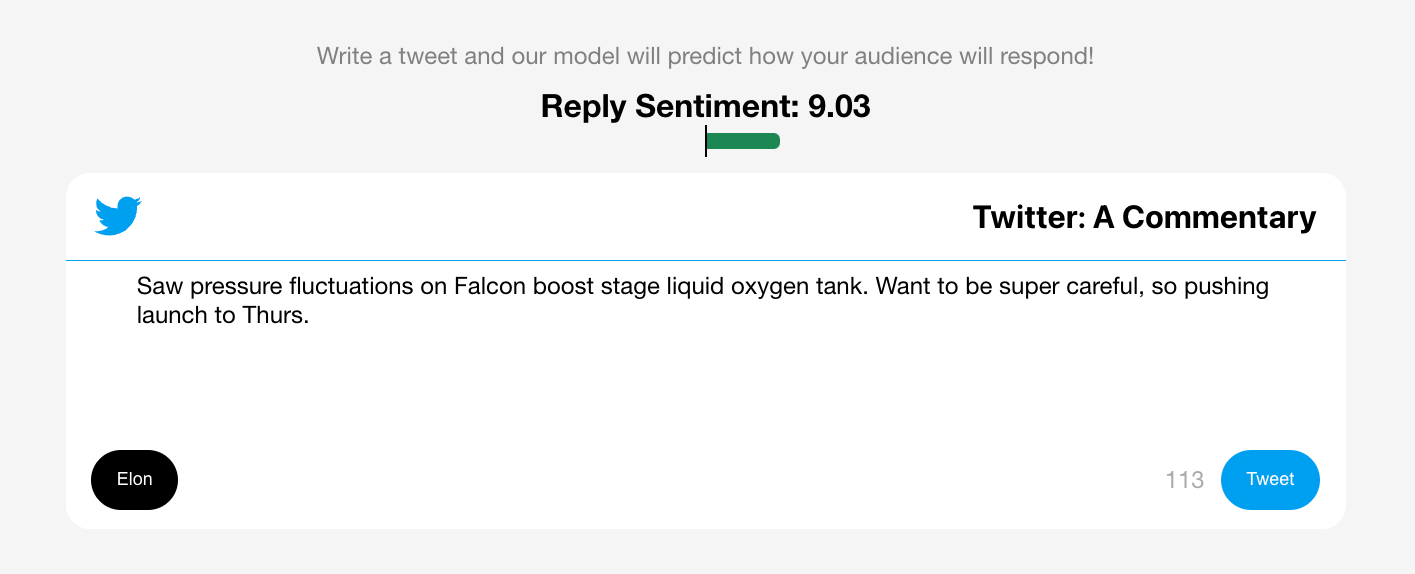
\includegraphics[width=1\textwidth]{product.png}
      \caption{Sample tweet and predicted sentiment from \href{https://twittercommentary.netlify.app/}{https://twittercommentary.netlify.app/}}
    \end{figure}

  \end{block}

  \begin{block}{Future Research}

    In the future, we would like to build a more robust model. Often, we noticed that the model could be easily skewed by the presence of certain words in the tweet with high prior probabilities like \code{love}. This could be combatted by training on a wider dataset or by using an n-gram model, which splits the data into $n$ word chunks to partially preserve the relationship between words that are next to each other. We would also like to make the model more easily interpretable by users since it is currently unclear which words affect the predicted sentiment the most.
  
  \end{block}

  \begin{block}{References}

    \footnotesize{\bibliographystyle{ieeetr}\bibliography{poster}}

  \end{block}

\end{column}

\separatorcolumn
\end{columns}
\end{frame}

\end{document}
